\section{Specific requirements}
%%%%%%%%%%%%%%%%%%%%%%%%%%%%%%%%%%%%%%%%%%%%%%%%%%%%%%%%%%%%%%%%%%%%%%%%%%%%%%%%
% This section of the SRS should contain all of the software requirements to a level of detail sufficient to enable designers to design a system to satisfy those requirements, and testers to test that the system satisfies those requirements.
% Throughout this section, every stated requirement should be externally perceivable by users, operators, or other external systems.
% These requirements should include at a minimum a description of every input (stimulus) into the system, every output (response) from the system, and all functions performed by the system in response to an input or in support of an output.
% As this is often the largest and most important part of the SRS, the following principles apply:
% Specific requirements should be stated in conformance with all the characteristics described in 4.3.
%   1. Specific requirements should be cross-referenced to earlier documents that relate.
%   2. All requirements should be uniquely identifiable.
%   3. Careful attention should be given to organizing the requirements to maximize readability.
% Before examining specific ways of organizing the requirements it is helpful to understand the various items that comprise requirements as described in 5.3.1 through 5.3.7.
%%%%%%%%%%%%%%%%%%%%%%%%%%%%%%%%%%%%%%%%%%%%%%%%%%%%%%%%%%%%%%%%%%%%%%%%%%%%%%%%

% \begin{enumerate}
%   \item You must have an XML declaration statement.
%     \begin{itemize}
%       \item \inlinecode{<?xml version="1.0" standalone="yes/no" encoding="UTF-8"?>}
%       \item {
%         The purpose of a declaration is to tell the browser or other handlers th at the document is an XML document.
%         The version in the declaration statement indicates the version of the XML specification that the document conforms to; standalone indicates whether the document is accompanied by a DTD file.
%       }
%     \end{itemize}
%     \item Is there a DTD file?
%       \begin{itemize} 
%         \item { 
%           The do cument must have a corresponding DTD file, and strictly comply with the DTD file specification.
%          The DTD file's declaration statement follows the XML declaration statement.
%           \inlinecode{<!DOCTYPE type-of-doc SYSTEM/PUBLIC "dtd-name">}
%         }
%       \end{itemize}
%     \item Note your capitalization
%         \begin{itemize}
%             \item In the XML file, the case is a difference.
%         \end{itemize} 
%     \item Quotes attributes values
%     \item All identifiers must have a corresponding end tag.
% \end{enumerate}

\subsection{External interfaces}
%%%%%%%%%%%%%%%%%%%%%%%%%%%%%%%%%%%%%%%%%%%%%%%%%%%%%%%%%%%%%%%%%%%%%%%%%%%%%%%%
% This should be a detailed description of all inputs into and outputs from the software system.
% It should complement the interface descriptions in 5.2 and should not repeat information there.
% It should include both content and format as follows:
%   - Name of item;
%   - Description of purpose;
%   - Source of input or destination of output;
%   - Valid range, accuracy, and/or tolerance;
%   - Units of measure;
%   - Timing;
%   - Relationships to other inputs/outputs;
%   - Screen formats/organization;
%   - Window formats/organization;
%   - Data formats;
%   - Command formats;
%   - End messages.
%%%%%%%%%%%%%%%%%%%%%%%%%%%%%%%%%%%%%%%%%%%%%%%%%%%%%%%%%%%%%%%%%%%%%%%%%%%%%%%%

XSLT40-Transformer will have two user interfaces: a \textbf{Web Interface} and a \textbf{Commandline Interface (CLI)}.

\begin{description}
    \item {
        \textbf{Web Interface}:
        The website interface for XZES40-Transformer will include of a form with the following fields:
        \begin{description}
            \item {
              \textbf{XML File} A file upload field for the XML document.
            }
            \item {
              \textbf{XSLT File} A file upload field for the XSLT document.
            }
            \item {
              \textbf{Output Filename} (optional)
              The filename of the output document.
              If one is not specified a name will be generated of the following format \inlinecode{document-transform-<date>.xml>}.
            }
%            \item {
%              \textbf{Username} (optional)
%              Specifies a user name if one is required.
%            }
%            \item {
%              \textbf{Password} (optional)
%              Specifies the user's password if one is required.
%            }
        \end{description}

        The website will make an HTTP \inlinecode{POST} request to the server.
        This \inlinecode{POST} request will include an XML and XSLT document in it's payload.

        The page will redirect the user to a new page where they can download the transformed file.

        The Web Interface will require a web-browser (supporting HTTP4.0+).
        
        \begin{figure}[h]
        \caption{Prototype of the Web Interface}
        \centering
        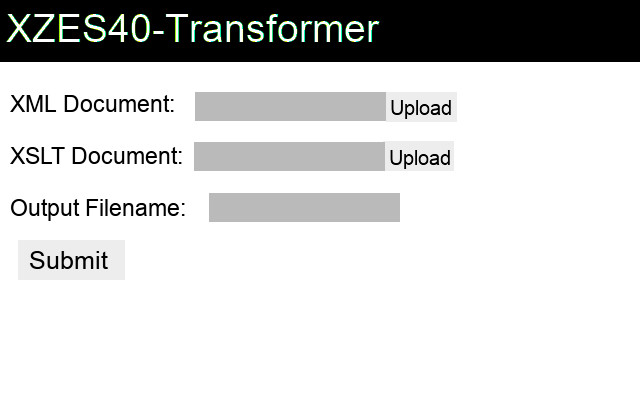
\includegraphics{figures/website-mockup.jpg}
        \end{figure}
    }
    \item {
        \textbf{Command-Line Interface (CLI)}:
        The CLI will give users a text-based interface with XZES40-Transformer.
        The with the following flags:
        \begin{description}
            \item {
              \textbf{\inlinecode{--xml-file=}}
              Specifies the input XML document.
            }
            \item {
              \textbf{\inlinecode{--xslt-file=}}
              Specifies the input XSLT document.
            }
            \item {
              \textbf{\inlinecode{--server=}}
              Specifies which server to connect to (\inlinecode{e.g., http://servername.ext})
            }
            \item {
              \textbf{\inlinecode{--output-file=}} (optional)
              Specifies a file to write out to.  Otherwise writes to a file of the following format \inlinecode{document-transform-<date>.xml>}.
            }
            \item {
              \textbf{\inlinecode{--port=}} (optional)
              Specifies which port to connect through if non-standard (\inlinecode{e.g., 8001})
            }
%            \item {
%              \textbf{\inlinecode{--username=}} (optional)
%              Specifies a user name if one is required.
%            }
%            \item {
%              \textbf{\inlinecode{--password=}} (optional)
%              Specifies the user's password if one is required.
%            }
            \item {
              \textbf{\inlinecode{--help=}} (optional)
              Prints out a help menu (describing these flags)
            }
        \end{description}

        The CLI will take the following arguments and make a \inlinecode{POST} request to the server.
        The transformed file will be automatically downloaded to the user's desired location, or to the current working directory with the automatic file name.

        The CLI requires a UNIX terminal and UNIX shell.
    }
    \begin{lstlisting}
    EXAMPLE OF CLI INTERFACE.
    \end{lstlisting}
\end{description}

Both interfaces XZES40-Transformer will require a method of input (keyboard, mouse, touchscreen, etc), an internet connection, and monitor or screen.

As input both interfaces expect one XML 1.0 formatted document and one XSLT 1.0 formatted document.
These files can be UTF-8 or ASCII character encoding.

As output both interfaces will send the user an XML 1.0 formatted document of UTF-8 character encoding.

% The system provides external interface, or system call external interface, often using XML format as the interface data transfer format.
% 
% \begin{enumerate}
%   \item The use of Xstream library can be directly javabean into XML file, of course, can also be XML file data into java bean.
%   \item {
%     Spring MVC + freemarker framework, get request to put the data into the ModelMap, dispatchServlet use freemarker template engine, the ModelMap data will be rendered to.
%     Ftl file, generate the page.
%     Use this principle, direct call freemarker template engine rendering method, the data is rendered to.
%     Ftl file, generate the required XML format data.
%   }
% \end{enumerate}

\subsection{Functions}
%%%%%%%%%%%%%%%%%%%%%%%%%%%%%%%%%%%%%%%%%%%%%%%%%%%%%%%%%%%%%%%%%%%%%%%%%%%%%%%%
% Functional requirements should define the fundamental actions that must take place in the software in accepting and processing the inputs and in processing and generating the outputs.
% These are generally listed as “shall” statements starting with “The system shall…”
% These include
%   - Validity checks on the inputs
%   - Exact sequence of operations
%   - Responses to abnormal situations, including
%     - Overflow
%     - Communication facilities
%     - Error handling and recovery
%   - Effect of parameters
%   - Relationship of outputs to inputs, including
%     - Input/output sequences
%     - Formulas for input to output conversion
% It may be appropriate to partition the functional requirements into subfunctions or subprocesses.
% This does not imply that the software design will also be partitioned that way.
%%%%%%%%%%%%%%%%%%%%%%%%%%%%%%%%%%%%%%%%%%%%%%%%%%%%%%%%%%%%%%%%%%%%%%%%%%%%%%%%

%\begin{itemize}
%  \item {
%   \inlinecode{string utf8\_decode (string \$data)}: 
%    This function decodes data encoded in UTF-8 to ISO-8859-1.
% }
% \item {
%    \inl\begin{itemize}
% \item {
%    \inlinecode{string utf8\_decode (string \$data)}: 
%    This function decodes data encoded in UTF-8 to ISO-8859-1.
%  }
%  \item {
%    \inlinecode{string utf8\_encode ( string \$data )}:
%    This function converts the data string to UTF-8 encoding and returns the encoded string.
%  }
%  \item {
%    \inlinecode{string xml\_error\_string ( int \$code )}:
%    Obtain an XML parser error string based on the given code.
%  }
%  \item{%   \inlinecode{int xml\_get\_current\_byte\_index ( resource \$parser )}:
%    Gets the current byte index of the specified XML parser
%  }
%  \item{
%    \inlinecode{int xml\_get\_current\_column\_number ( resource \$parser )}
%    Gets the current column number of the specified XML parser
%  }
%  \item{
%    \inlinecode{int xml\_get\_current\_line\_number ( resource \$parser )}
%    Gets the current line number of the specified XML parser
%  }
%  \item{
%    \inlinecode{int xml\_parse\_into\_struct ( resource \$parser , string \$data , array \&\$values [, array \&\$index ] )}
%    This function parses the XML file into two corresponding arrays, and the index parameter contains a pointer to the corresponding value in the values array.
%   The last two array parameters can be passed to the function by the pointer.
% }
%  \item{
%    \inlinecode{int xml\_parse ( resource \$parser , string \$data [, bool \$is\_final = false ] )}
%    Xml\_parse () Parses an XML document.
%    The handler for the configured event is called indefinitely as needed
%  }
%\end{itemize}inecode{string utf8\_encode ( string \$data )}:
%   This function converts the data string to UTF-8 encoding and returns the encoded string.
%  }
%  \item {
%    \inlinecode{string xml\_error\_string ( int \$code )}:
%    Obtain an XML parser error string based on the given code.
%  }
 % \item{
  %  \inlinecode{int xml\_get\_current\_byte\_index ( resource \$parser )}:
   % Gets the current byte index of the specified XML parser
%  }
% \item{
%    \inlinecode{int xml\_get\_current\_column\_number ( resource \$parser )}
%    Gets the current column number of the specified XML parser
%  }
%  \item{
%    \inlinecode{int xml\_get\_current\_line\_number ( resource \$parser )}
%    Gets the current line number of the specified XML parser
%  }
%  \item{
%    \inlinecode{int xml\_parse\_into\_struct ( resource \$parser , string \$data , array \&\$values [, array \&\$index ] )}
%    This function parses the XML file into two corresponding arrays, and the index parameter contains a pointer to the corresponding value in the values array.
%    The last two array parameters can be passed to the function by the pointer.
%  }
%  \item{
%   \inlinecode{int xml\_parse ( resource \$parser , string \$data [, bool \$is\_final = false ] )}
%    Xml\_parse () Parses an XML document.
%   The handler for the configured event is called indefinitely as needed
%  }
%\end{itemize}

The following functions will be the core functionality of XZES40-Transformer.

\begin {itemize}
    \item{
        \inlinecode{int verify\_file(string input\_filename, int format\_option)}:
        Open file and verify that it is the correct format (XML 1.0 or XSLT 1.0).

        Returns FILE\_ERROR value if the file cannot be found, FORMAT\_ERROR if the given file is not of the correct format, and VALID if the file is of the correct format.
        Each return value will be a macro for a unique integer value.
    }
    \item{
        \inlinecode{void transform(string XML\_filename, string XSLT\_filename, string output\_filename)}:
        % After the server verifies the XML and XSLT file are correct format, the system will transform those files.
        This function is called to transform the given XML\_FILE with the XSLT\_FILE.
        If output\_file is defined the file will be written to that location.
        If output\_file is not defined the new file will be written to STDOUT.
    }
    \item{
        \inlinecode{char * verify_cache(input\_filename)}:
        Ensures that a given file is cached.
        Adds the file to cache if it is not already.
        Returns a pointer to the cached file.
    }
    \item{
        \inlinecode{int check\_cache(input\_filename)}:
        The system will check if the given file is in the cache.
        
        Returns TRUE if the file is in the cache and FALSE if the file is not in the cache.
    }
    \item{
        \inlinecode{int cache(input\_filename)}:
        The new XML file will be saved in the cache.
        
        Returns SUCCESS if the document was successfully cached, FALSE if it was not successfully cached.
    }
    \item{
        \inlinecode{int compile(input\_filename)}:
        The system will compile the given XML/XSLT file into machine code to later be transformed.
    }
    \item{
        \inlinecode{int perform\_transform(var1, var2)}:
        Performs the document transformation.
    }
    \item{
        \inlinecode{int clean_cache()}:
        Removes old documents from the cache which have not been used recently.
    }
\end{itemize}

\subsection{Performance requirements}
%%%%%%%%%%%%%%%%%%%%%%%%%%%%%%%%%%%%%%%%%%%%%%%%%%%%%%%%%%%%%%%%%%%%%%%%%%%%%%%%
% This subsection should specify both the static and the dynamic numerical requirements placed on the software or on human interaction with the software as a whole.
% Static numerical requirements may include the following:
%   1. The number of terminals to be supported;
%   2. The number of simultaneous users to be supported;
%   3. Amount and type of information to be handled.
% Static numerical requirements are sometimes identified under a separate section entitled Capacity.
% Dynamic numerical requirements may include, for example, the numbers of transactions and tasks and the amount of data to be processed within certain time periods for both normal and peak workload conditions.
% All of these requirements should be stated in measurable terms.
% For example:
%
% 95% of the transactions shall be processed in less than 1 s.
% rather than,
% An operator shall not have to wait for the transaction to complete.
% Numerical limits applied to one specific function are normally specified as part of the processing subparagraph description of that function.
%%%%%%%%%%%%%%%%%%%%%%%%%%%%%%%%%%%%%%%%%%%%%%%%%%%%%%%%%%%%%%%%%%%%%%%%%%%%%%%%

% XZES40-Transformer application will support 3 or 4 terminals at the same time, and we expect 3 or 4 simultaneous users to be supported.
% XZES40-Transformer application can handle XML and XSLT file.(?) 

XZES40-Transformer will support X transformations per second and Y concurrent users with Z latency.
    
%\begin{enumerate}
%    \item DOM( Document Object Model)
%    \begin{itemize}
%        \item {
%          The DOM is the official W3C standard for representing XML documents in a platform-independent and language-independent manner.
%          A DOM is a collection of nodes or pieces of information organized in a hierarchical structure.
%          This hierarchy allows the developer to find specific information in the tree.
%          Analysis of the structure is usually required to load the entire document and structure hierarchy, and then to do any work.
%          Because it is based on the level of information, so DOM is considered to be tree-based or object-based.
%        }
%    \end{itemize}
%    \item SAX (Simple API for XML)
%    \begin{itemize}
%        \item {
%          Analysis can start immediately, rather than waiting for all the data to be processed.
%          Also, because the application only checks data when reading data, there is no need to store the data in memory.
%          This is a huge advantage for large documents.
%          In fact, the application does not even have to parse the entire document; it can stop resolving when a condition is met.
%       }
%    \end{itemize}
%    \item JDOM(Java-based Document Object Model)
%    \begin{itemize}
%        \item The goal of JDOM is to become a Java-specific document model that simplifies interaction with XML and is faster than using the DOM implementation.
%    \end{itemize}
%    \item DOM4J(Document Object Model for Java)
%    \begin{itemize}
%        \item {
%          Although DOM4J represents a completely independent development results, but initially, it is a smart JDOM branch.
%          It incorporates a number of features beyond the basic XML document representation, including integrated XPath support, XML Schema support, and event-based processing for large documents or fluidized documents.
%          It also provides the option of building document representations that have parallel access through the DOM4J API and the standard DOM interface.
%        }
%    \end{itemize}
%\end{enumerate}


\subsection{Logical database requirements}
%%%%%%%%%%%%%%%%%%%%%%%%%%%%%%%%%%%%%%%%%%%%%%%%%%%%%%%%%%%%%%%%%%%%%%%%%%%%%%%%
% This should specify the logical requirements for any information that is to be placed into a database.
% This may include the following:
%   1. Types of information used by various functions;
%   2. Frequency of use;
%   3. Accessing capabilities;
%   4. Data entities and their relationships;
%   5. Integrity constraints;
%   6. Data retention requirements.
%%%%%%%%%%%%%%%%%%%%%%%%%%%%%%%%%%%%%%%%%%%%%%%%%%%%%%%%%%%%%%%%%%%%%%%%%%%%%%%%

XZES40-Transformer application does not require database. 

\subsection{Design constraints}
%%%%%%%%%%%%%%%%%%%%%%%%%%%%%%%%%%%%%%%%%%%%%%%%%%%%%%%%%%%%%%%%%%%%%%%%%%%%%%%%
% This should specify design constraints that can be imposed by other standards, hardware limitations, etc.
%%%%%%%%%%%%%%%%%%%%%%%%%%%%%%%%%%%%%%%%%%%%%%%%%%%%%%%%%%%%%%%%%%%%%%%%%%%%%%%%

% In XML technology, you can write a document to constrain an XML document writing specification, which is called XML constraints.
% In XML Schema technology has a technical term to describe the process, the XML Schema document declaration element binding to a namespace, after the XML file through the URI which is namespace to tell the parsing engine, XML document In the preparation of the elements from where, who is bound.
% DTD (Document Type Definition)
% The XML file uses the DOCTYPE declaration statement to specify the DTD file it follows.

For the XML compilation and transformation process we are restricted to using the Xerces-C and Xalan-C libraries.
For document encoding and decoding we have to use the ICU UTF-8 libary.

% OS restriction?

\subsubsection{Standards Compliance}
%%%%%%%%%%%%%%%%%%%%%%%%%%%%%%%%%%%%%%%%%%%%%%%%%%%%%%%%%%%%%%%%%%%%%%%%%%%%%%%%
% This subsection should specify the requirements derived from existing standards or regulations.
% They may include the following:
%   1. Report format;
%   2. Data naming;
%   3. Accounting procedures;
%   4. Audit tracing.
% For example, this could specify the requirement for software to trace processing activity.
% Such traces are needed for some applications to meet minimum regulatory or financial standards.
% An audit trace requirement may, for example, state that all changes to a payroll database must be recorded in a trace file with before and after values.
%%%%%%%%%%%%%%%%%%%%%%%%%%%%%%%%%%%%%%%%%%%%%%%%%%%%%%%%%%%%%%%%%%%%%%%%%%%%%%%%

Input documents must be correctly formatted XML and XSLT documents.
Malformed documents will be rejected by the application.

Correctly formatted XML documents follow the W3C outlined XML 1.0 and XSLT 1.0 formats. \cite{xml-spec} \cite{xslt-spec}

Our application will also communicate with users over HTTP/HTTPS, however we are not implementing these standards, just using them to communicate over the internet.

%The XML declaration typically appears as the first line in an XML document.
%The XML declaration is not required, however, if used it must be the first line in the document and no other content or white space can precede it.
%\begin{enumerate}
%    \item The version number, <?xml version="1.0"?>
%    \begin{itemize}
%        \item {
%          This is mandatory.
%          Although the number might change for future versions of XML, 1.0 is the current version.
%        }
%    \end{itemize}
%    \item The encoding declaration, <?xml version="1.0" encoding="UTF-8"?>
%    \begin{itemize}
%        \item {
%          This is optional.
%          If used, the encoding declaration must appear immediately after the version information in the XML declaration, and must contain a value representing an existing character encoding.
%        }
%    \end{itemize}
%\end{enumerate}

\subsection{Software System Attributes}
%%%%%%%%%%%%%%%%%%%%%%%%%%%%%%%%%%%%%%%%%%%%%%%%%%%%%%%%%%%%%%%%%%%%%%%%%%%%%%%%
% There are a number of attributes of software that can serve as requirements.
% It is important that required attributes be specified so that their achievement can be objectively verified.
% Subclauses 5.3.6.1 through 5.3.6.5 provide a partial list of examples.
%%%%%%%%%%%%%%%%%%%%%%%%%%%%%%%%%%%%%%%%%%%%%%%%%%%%%%%%%%%%%%%%%%%%%%%%%%%%%%%%

% XML elements can include attributes in the opening tag, similar to HTML.

\subsubsection{Reliability}
%%%%%%%%%%%%%%%%%%%%%%%%%%%%%%%%%%%%%%%%%%%%%%%%%%%%%%%%%%%%%%%%%%%%%%%%%%%%%%%%
% This should specify the factors required to establish the required reliability of the software system at time of delivery.
%%%%%%%%%%%%%%%%%%%%%%%%%%%%%%%%%%%%%%%%%%%%%%%%%%%%%%%%%%%%%%%%%%%%%%%%%%%%%%%%

For XZES40-Transformer to be reliable will require it's cache to be up to date, to avoid transforming documents incorrectly.

% The XML test case model is put forward by using XML to save the test cases generated in the software reliability test.
% The XML test case file generator and test engine are implemented, and the test cases are read with the test driver to drive the tested program to run.
% Test Results.
% Which can automatically and efficiently test the software interface.
% The test data is separated from the test driver, 
% which is beneficial to the maintenance and reuse of the test data, and has achieved very good results in practical application.

\subsubsection{Availability}
%%%%%%%%%%%%%%%%%%%%%%%%%%%%%%%%%%%%%%%%%%%%%%%%%%%%%%%%%%%%%%%%%%%%%%%%%%%%%%%%
% This should specify the factors required to guarantee a defined availability level for the entire system such as checkpoint, recovery, and restart.
%%%%%%%%%%%%%%%%%%%%%%%%%%%%%%%%%%%%%%%%%%%%%%%%%%%%%%%%%%%%%%%%%%%%%%%%%%%%%%%%

Since XZES40-Transformer will be run as a web-service it should be highly-available during business hours.
It will be configured to handle heavy workloads and restart if it crashes.

% XML provides a way to describe data and platform-independent,
% has become the de facto standard for data exchange on the Internet.

\subsubsection{Security}
%%%%%%%%%%%%%%%%%%%%%%%%%%%%%%%%%%%%%%%%%%%%%%%%%%%%%%%%%%%%%%%%%%%%%%%%%%%%%%%%
% This should specify the factors that protect the software from accidental or malicious access, use, modification, destruction, or disclosure.
% Specific requirements in this area could include the need to
%    1. Utilize certain cryptographical techniques;
%    2. Keep specific log or history data sets;
%    3. Assign certain functions to different modules;
%    4. Restrict communications between some areas of the program;
%    5. Check data integrity for critical variables.
%%%%%%%%%%%%%%%%%%%%%%%%%%%%%%%%%%%%%%%%%%%%%%%%%%%%%%%%%%%%%%%%%%%%%%%%%%%%%%%%

XZES40-Transformer may be used to handle sensitive data, however it is not this team's job to account for that.

If administrators want the application to be secure they may choose to deploy it behind an organization firewall or configure the web-service to use HTTPS instead of HTTP.

% XML encryption provides an end-to-end security for applications that require secure data exchange of structured data.
% XML itself is the most popular technique for structuring data, so XML-based encryption becomes a method of dealing with the complex requirements of security in data interchange applications.

\subsubsection{Maintainability}
%%%%%%%%%%%%%%%%%%%%%%%%%%%%%%%%%%%%%%%%%%%%%%%%%%%%%%%%%%%%%%%%%%%%%%%%%%%%%%%%
% This should specify attributes of software that relate to the ease of maintenance of the software itself.
% There may be some requirement for certain modularity, interfaces, complexity, etc.
% Requirements should not be placed here just because they are thought to be good design practices.
%%%%%%%%%%%%%%%%%%%%%%%%%%%%%%%%%%%%%%%%%%%%%%%%%%%%%%%%%%%%%%%%%%%%%%%%%%%%%%%%

Our application will also be deployed as a daemon which will be configured on installation.

% In the design of the time, if some of the key parameters into the configuration file, can be used for software deployment and bring more flexibility.

\subsubsection{Portability}
%%%%%%%%%%%%%%%%%%%%%%%%%%%%%%%%%%%%%%%%%%%%%%%%%%%%%%%%%%%%%%%%%%%%%%%%%%%%%%%%
% This should specify attributes of software that relate to the ease of porting the software to other host machines and/or operating systems.
% This may include the following:
%%%%%%%%%%%%%%%%%%%%%%%%%%%%%%%%%%%%%%%%%%%%%%%%%%%%%%%%%%%%%%%%%%%%%%%%%%%%%%%%
% Some systems provide different sets of functions to different classes of users.
% For example, an elevator control system presents different capabilities to passengers, maintenance workers, and fire fighters.
% When organizing this section by user class, the outline in A.3 should be used.
%%%%%%%%%%%%%%%%%%%%%%%%%%%%%%%%%%%%%%%%%%%%
%    1. Percentage of components with host-dependent code;
%    2. Percentage of code that is host dependent;
%    3. Use of a proven portable language;
%    4. Use of a particular compiler or language subset;
%    5. Use of a particular operating system.
%%%%%%%%%%%%%%%%%%%%%%%%%%%%%%%%%%%%%%%%%%%%%%%%%%%%%%%%%%%%%%%%%%%%%%%%%%%%%%%%

As an Open Source project XZES40-Transformer will be designed for portability.
It will perform all operating-system specific operations via an OS agnostic API.
When the application is compiled on a new platform it will compile against the given OS api (Windows, Linux, MacOS, etc).

% A DTD, such as the priceList DTD, is what gives XML data its portability.
% If an application is sent a priceList document in XML format and has the priceList DTD, 
% it can process the document according to the rules specified in the DTD.

\subsection{Organizing the specific requirements}
%%%%%%%%%%%%%%%%%%%%%%%%%%%%%%%%%%%%%%%%%%%%%%%%%%%%%%%%%%%%%%%%%%%%%%%%%%%%%%%%
% For anything but trivial systems the detailed requirements tend to be extensive.
% For this reason, it is recommended that careful consideration be given to organizing these in a manner optimal for understanding.
% There is no one optimal organization for all systems.
% Different classes of systems lend themselves to different organizations of requirements in Section 3 of the SRS.
% Some of these organizations are described in 5.3.7.1 through 5.3.7.7.
%%%%%%%%%%%%%%%%%%%%%%%%%%%%%%%%%%%%%%%%%%%%%%%%%%%%%%%%%%%%%%%%%%%%%%%%%%%%%%%%

%\begin{enumerate}
%    \item The file must be in Unicode Convert Format -8 (UTF-8).
%    \item {
%      The file must have a unique migration urlid.
%      The urlid you specify for each file in the command line must be different.
%      If two migrated .xml files have the same urlid, the second .xml file specified on the command line will not be processed.
%    The reason for this is that USMT uses the urlid to define the components in the file.
%   }
%   \item Each component in the file must have a display name for display in the Config.xml file.
%\end{enumerate}

\subsubsection{System mode}
%%%%%%%%%%%%%%%%%%%%%%%%%%%%%%%%%%%%%%%%%%%%%%%%%%%%%%%%%%%%%%%%%%%%%%%%%%%%%%%%
% Some systems behave quite differently depending on the mode of operation.
% For example, a control system may have different sets of functions depending on its mode: training, normal, or emergency.
% When organizing this section by mode, the outline in A.1 or A.2 should be used.
% The choice depends on whether interfaces and performance are dependent on mode.
%%%%%%%%%%%%%%%%%%%%%%%%%%%%%%%%%%%%%%%%%%%%%%%%%%%%%%%%%%%%%%%%%%%%%%%%%%%%%%%%

Our application will behave the same in all modes.
Given a \inlinecode{POST} request to the server it will respond with a file.

% \begin{enumerate}
%     \item The file must be in Unicode Convert Format -8 (UTF-8).
%     \item {
%       The file must have a unique migration urlid.
%       The urlid you specify for each file in the command line must be different.
%       If two migrated .xml files have the same urlid, the second .xml file specified on the command line will not be processed.
%       The reason for this is that USMT uses the urlid to define the components in the file.
%     }
%     \item Each component in the file must have a display name for display in the Config.xml file.
% \end{enumerate}

\subsubsection{User class}
%%%%%%%%%%%%%%%%%%%%%%%%%%%%%%%%%%%%%%%%%%%%%%%%%%%%%%%%%%%%%%%%%%%%%%%%%%%%%%%%
% Some systems provide different sets of functions to different classes of users.
% For example, an elevator control system presents different capabilities to passengers, maintenance workers, and fire fighters.
% When organizing this section by user class, the outline in A.3 should be used.
%%%%%%%%%%%%%%%%%%%%%%%%%%%%%%%%%%%%%%%%%%%%%%%%%%%%%%%%%%%%%%%%%%%%%%%%%%%%%%%%

Our application does not differentiate between different users, each user will receive the same functionality.

% A user-defined simple type is a restriction on the content of an element or attribute.
% A user-defined simple type always limits the content of the element to a subset of the existing simple types that the element exports

\subsubsection{Objects}
%%%%%%%%%%%%%%%%%%%%%%%%%%%%%%%%%%%%%%%%%%%%%%%%%%%%%%%%%%%%%%%%%%%%%%%%%%%%%%%%
% Objects are real-world entities that have a counterpart within the system.
% For example, in a patient monitoring system, objects include patients, sensors, nurses, rooms, physicians, medicines, etc.
% Associated with each object is a set of attributes (of that object) and functions (performed by that object).
% These functions are also called services, methods, or processes.
% When organizing this section by object, the outline in A.4 should be used.
% Note that sets of objects may share attributes and services.
% These are grouped together as classes.
%%%%%%%%%%%%%%%%%%%%%%%%%%%%%%%%%%%%%%%%%%%%%%%%%%%%%%%%%%%%%%%%%%%%%%%%%%%%%%%%

The system will have one object, cached files.
Each input file will be compiled and cached with metadata about the file like when the cache was created, when it was last used, the filename, and the compiled file contents.
The object will be accessed from the cache by indexing the file's hash.

For example:
\begin{lstlisting}[language=c]
struct document {
  char * filename;
  int created;
  int accessed;
  void * cached-content;
}
\end{lstlisting}

% The Element object represents an element in an XML document.
% Elements may contain attributes, other elements, or text.
% If an element contains text, the text is represented in a text-node.

\subsubsection{Feature}
%%%%%%%%%%%%%%%%%%%%%%%%%%%%%%%%%%%%%%%%%%%%%%%%%%%%%%%%%%%%%%%%%%%%%%%%%%%%%%%%
% A feature is an externally desired service by the system that may require a sequence of inputs to effect the desired result.
% For example, in a telephone system, features include local call, call forwarding, and conference call.
% Each feature is generally described in a sequence of stimulus-response pairs.
% When organizing this section by feature, the outline in A.5 should be used.
%%%%%%%%%%%%%%%%%%%%%%%%%%%%%%%%%%%%%%%%%%%%%%%%%%%%%%%%%%%%%%%%%%%%%%%%%%%%%%%%

The core feature of our application is that it accepts an XML and XSLT document and returns a transformed XML document.

Caching

Parallel computation

% XML is a text format to describe a file format
% Because XML is described in text form, it is suitable for data exchange in various platform environments.
% Similarly, the use of text to describe the content, you can cross the barriers of different platforms for normal data exchange.

\subsubsection{Stimulus}
%%%%%%%%%%%%%%%%%%%%%%%%%%%%%%%%%%%%%%%%%%%%%%%%%%%%%%%%%%%%%%%%%%%%%%%%%%%%%%%%
% Some systems can be best organized by describing their functions in terms of stimuli.
% For example, the functions of an automatic aircraft landing system may be organized into sections for loss of power, wind shear, sudden change in roll, vertical velocity excessive, etc.
% When organizing this section by stimulus, the outline in A.6 should be used.
%%%%%%%%%%%%%%%%%%%%%%%%%%%%%%%%%%%%%%%%%%%%%%%%%%%%%%%%%%%%%%%%%%%%%%%%%%%%%%%%

Our system has two responses to stimulus:

1. 

% We can AXIOM stimulus XML.
% It has a clear design goal: a substantial increase Apache next-generation SOAP protocol stack Axis 2 performance.
% The result is AXIOM (also called OM), which is different from other object models, because it highlights the lightness of the construct and is built only when needed.
% Because it is lightweight, it minimizes the stress on system resources, especially the CPU and memory.
% At the same time, deferred construction allows the use of a portion of the tree when other parts are not yet complete.

\subsubsection{Response}
%%%%%%%%%%%%%%%%%%%%%%%%%%%%%%%%%%%%%%%%%%%%%%%%%%%%%%%%%%%%%%%%%%%%%%%%%%%%%%%%
% Some systems can be best organized by describing all the functions in support of the generation of a response.
% For example, the functions of a personnel system may be organized into sections corresponding to all functions associated with generating paychecks, all functions associated with generating a current list of employees, etc.
% The outline in A.6 (with all occurrences of stimulus replaced with response) should be used.
%%%%%%%%%%%%%%%%%%%%%%%%%%%%%%%%%%%%%%%%%%%%%%%%%%%%%%%%%%%%%%%%%%%%%%%%%%%%%%%%

% Flag the status of the entire software operation.
% Only when the service response code is 2000, it means that the software for the actual data analysis and processing operations.
% When the service response code is a different value, it means that due to various exceptions, the software does not carry out actual data analysis and processing, which is equivalent to an error in the system periphery.

\subsubsection{Functional hierarchy}
%%%%%%%%%%%%%%%%%%%%%%%%%%%%%%%%%%%%%%%%%%%%%%%%%%%%%%%%%%%%%%%%%%%%%%%%%%%%%%%%
% When none of the above organizational schemes prove helpful, the overall functionality can be organized into a hierarchy of functions organized by either common inputs, common outputs, or common internal data access.
% Data flow diagrams and data dictionaries can be used to show the relationships between and among the functions and data.
% When organizing this section by functional hierarchy, the outline in A.7 should be used.
%%%%%%%%%%%%%%%%%%%%%%%%%%%%%%%%%%%%%%%%%%%%%%%%%%%%%%%%%%%%%%%%%%%%%%%%%%%%%%%%

% Root element->element->attribute “category”->text
%need more information

\subsection{Additional comments}
%%%%%%%%%%%%%%%%%%%%%%%%%%%%%%%%%%%%%%%%%%%%%%%%%%%%%%%%%%%%%%%%%%%%%%%%%%%%%%%%
% Whenever a new SRS is contemplated, more than one of the organizational techniques given in 5.3.7.7 may be appropriate.
% In such cases, organize the specific requirements for multiple hierarchies tailored to the specific needs of the system under specification.
% For example, see A.8 for an organization combining user class and feature.
% Any additional requirements may be put in a separate section at the end of the SRS.
%
% There are many notations, methods, and automated support tools available to aid in the documentation of requirements.
% For the most part, their usefulness is a function of organization.
% For example, when organizing by mode, finite state machines or state charts may prove helpful; when organizing by object, object-oriented analysis may prove helpful; when organizing by feature, stimulus-response sequences may prove helpful; and when organizing by functional hierarchy, data flow diagrams and data dictionaries may prove helpful.
%
% In any of the outlines given in A.1 through A.8, those sections called “Functional Requirement i” may be described in native language (e.g., English), in pseudocode, in a system definition language, or in four subsections titled: Introduction, Inputs, Processing, and Outputs.
%%%%%%%%%%%%%%%%%%%%%%%%%%%%%%%%%%%%%%%%%%%%%%%%%%%%%%%%%%%%%%%%%%%%%%%%%%%%%%%%

% XML has been widely used in document processing, data storage, Web applications (such as ajax data transmission, template application) and so on.
% As a structured language, it overcomes the shortcomings of the usual markup language markup fixes, and you can define your own markup to organize your data according to your own wishes.
% You can define DTDs and XML Schemas to make sure that your XML documents meet your requirements.
% XSLT can be used to XML documents according to a certain syntax into the document you need.

